\documentclass[12pt]{article}
\usepackage[danish]{babel}
\usepackage{amsfonts, amssymb, mathtools, amsthm, amsmath}
\usepackage{graphicx, pgfplots}
\usepackage{url}
\usepackage[dvipsnames]{xcolor}
\usepackage{sagetex}
\usepackage{lastpage}
\usepackage{wrapfig} 
\usepackage[stretch=10]{microtype} 

%loaded last
\usepackage[hidelinks]{hyperref}

\usepackage{siunitx}
  \sisetup{exponent-product = \cdot,
    output-decimal-marker = {,}}

%Giles Castelles incfig
\usepackage{import}
\usepackage{xifthen}
\usepackage{pdfpages}
\usepackage{transparent}

\newcommand{\incfig}[2][1]{%
  \def\svgwidth{#1\columnwidth}
  \import{../figures/}{#2.pdf_tex}
}

\setlength{\parindent}{0in}
\setlength{\oddsidemargin}{0in}
\setlength{\textwidth}{6.5in}
\setlength{\textheight}{8.8in}
\setlength{\topmargin}{0in}
\setlength{\headheight}{18pt}

\usepackage{fancyhdr}
\pagestyle{fancy}

\fancyhead{}
\fancyfoot{}
\fancyfoot[R]{Side \thepage{} af \pageref{LastPage}}
\fancyhead[L]{\footnotesize{Noah Rahbek Bigum Hansen}}

% Redefine the plain page style to be consistent
\fancypagestyle{plain}{
  \fancyhead{} % Clears all header content
  \fancyfoot{} % Clears all footer content
  \renewcommand{\headrulewidth}{0pt} % Removes the horizontal line
  \fancyfoot[R]{Side \thepage{} af \pageref{LastPage}} % Page number in the footer
}

\pgfplotsset{compat=newest}

\pgfplotsset{every axis/.append style={
  axis x line=middle,    % put the x axis in the middle
  axis y line=middle,    % put the y axis in the middle
  axis line style={<->,color=black}, % arrows on the axis
}}

\usepackage{thmtools}
\usepackage{tcolorbox}
  \tcbuselibrary{skins, breakable}
  \tcbset{
    space to upper=1em,
    space to lower=1em,
  }

\theoremstyle{definition}

\newtcolorbox[auto counter]{definition}[1][]{%
  breakable,
  colframe=ForestGreen,  %frame color
  colback=ForestGreen!5, %background color
  colbacktitle=ForestGreen!25, %background color for title
  coltitle=ForestGreen!70!black,  %title color
  fonttitle=\bfseries\sffamily, %title font
  left=1em,              %space on left side in box,
  enhanced,              %more options
  frame hidden,          %hide frame
  borderline west={2pt}{0pt}{ForestGreen},  %display left line
  title=Definition \thetcbcounter: #1,
}

\newtcolorbox{greenline}{%
  breakable,
  colframe=ForestGreen,  %frame color
  colback=white,          %remove background color
  left=1em,              %space on left side in box
  enhanced,              %more options
  frame hidden,          %hide frame
  borderline west={2pt}{0pt}{ForestGreen},  %display left line
}

\newtcolorbox[auto counter, number within=section]{eks}[1][]{%
  brekable,
  colframe=NavyBlue,  %frame color
  colback=NavyBlue!5, %background color
  colbacktitle=NavyBlue!25,    %background color for title
  coltitle=NavyBlue!70!black,  %title color
  fonttitle=\bfseries\sffamily, %title font
  left=1em,            %space on left side in box,
  enhanced,            %more options
  frame hidden,        %hide frame
  borderline west={2pt}{0pt}{NavyBlue},  %display left line
  title=Eksempel \thetcbcounter: #1
}

\newtcolorbox{blueline}{%
  breakable,
  colframe=NavyBlue,     %frame color
  colback=white,         %remove background
  left=1em,              %space on left side in box,
  enhanced,              %more options
  frame hidden,          %hide frame
  borderline west={2pt}{0pt}{NavyBlue},  %display left line
}

\newtcolorbox{teo}[1][]{%
  breakable,
  colframe=RawSienna,  %frame color
  colback=RawSienna!5, %background color
  colbacktitle=RawSienna!25,    %background color for title
  coltitle=RawSienna!70!black,  %title color
  fonttitle=\bfseries\sffamily, %title font
  left=1em,              %space on left side in box,
  enhanced,              %more options
  frame hidden,          %hide frame
  borderline west={2pt}{0pt}{RawSienna},  %display left line
  title=Teori: #1,
}

\newtcolorbox[auto counter, number within=section]{sæt}[1][]{%
  breakable,
  colframe=RawSienna,  %frame color
  colback=RawSienna!5, %background color
  colbacktitle=RawSienna!25,    %background color for title
  coltitle=RawSienna!70!black,  %title color
  fonttitle=\bfseries\sffamily, %title font
  left=1em,              %space on left side in box,
  enhanced,              %more options
  frame hidden,          %hide frame
  borderline west={2pt}{0pt}{RawSienna},  %display left line
  title=Sætning \thetcbcounter: #1,
  before lower={\textbf{Bevis:}\par\vspace{0.5em}},
  colbacklower=RawSienna!25,
}

\newtcolorbox{redline}{%
  breakable,
  colframe=RawSienna,  %frame color
  colback=white,       %Remove background color
  left=1em,            %space on left side in box,
  enhanced,            %more options
  frame hidden,        %hide frame
  borderline west={2pt}{0pt}{RawSienna},  %display left line
}

\newtcolorbox{for}[1][]{%
  breakable,
  colframe=NavyBlue,  %frame color
  colback=NavyBlue!5, %background color
  colbacktitle=NavyBlue!25,    %background color for title
  coltitle=NavyBlue!70!black,  %title color
  fonttitle=\bfseries\sffamily, %title font
  left=1em,              %space on left side in box,
  enhanced,              %more options
  frame hidden,          %hide frame
  borderline west={2pt}{0pt}{NavyBlue},  %display left line
  title=Forklaring #1,
}

\newtcolorbox{bem}{%
  breakable,
  colframe=NavyBlue,  %frame color
  colback=NavyBlue!5, %background color
  colbacktitle=NavyBlue!25,    %background color for title
  coltitle=NavyBlue!70!black,  %title color
  fonttitle=\bfseries\sffamily, %title font
  left=1em,              %space on left side in box,
  enhanced,              %more options
  frame hidden,          %hide frame
  borderline west={2pt}{0pt}{NavyBlue},  %display left line
  title=Bemærkning:,
}

\makeatother
\def\@lecture{}%
\newcommand{\lecture}[3]{
  \ifthenelse{\isempty{#3}}{%
    \def\@lecture{Lecture #1}%
  }{%
    \def\@lecture{Lecture #1: #3}%
  }%
  \subsection*{\makebox[\textwidth][l]{\@lecture \hfill \normalfont\small\textsf{#2}}}
}

\makeatletter

\newcommand{\opgave}[1]{%
 \def\@opgave{#1}%
 \subsection*{Opgave #1}
}

\makeatother

%Format lim the same way in intext and in display
\let\svlim\lim\def\lim{\svlim\limits}

% horizontal rule
\newcommand\hr{
\noindent\rule[0.5ex]{\linewidth}{0.5pt}
}

\title{Afleveringsopgave 6}
\author{Noah Rahbek Bigum Hansen}
\date{21. November 2024}

\begin{document}

\maketitle

\section*{Problem 1/3}

\begin{wrapfigure}[7]{r}{5.5cm}
  \vspace{-40pt}
  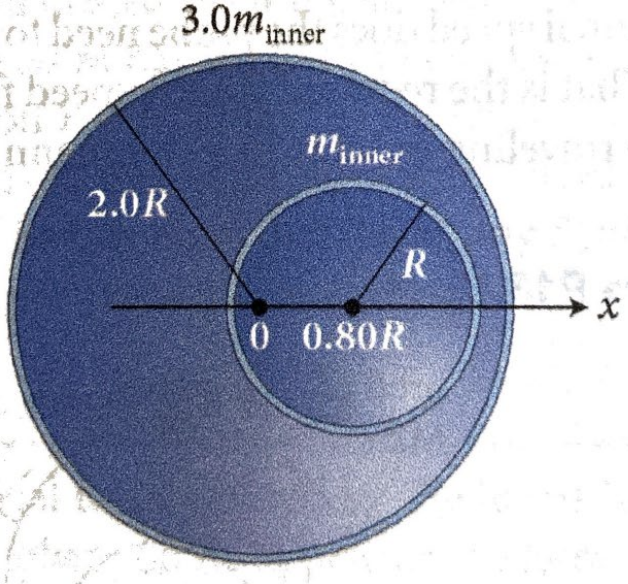
\includegraphics[width=5.5cm]{../figures/A2_1.png}
  \caption{}
  \label{fig:A2_1}
\end{wrapfigure}

Two uniform spherical shells are located such that their centers are along the $x$-xis in \textbf{\autoref{fig:A2_1}}. The inner shell has mass $m_{inner}$ and radius $R$, and its center is at $x = \num{0,80}R$. The outer shell has mass $\num{3,0} m_{inner}$ and radius $\num{2,0} R$, and its center is at $x = 0$. What is the magnitude of the vector sum of the gravitational forces exerted by these two shells on an object of mass $m_{obj}$ placed

\subsection*{(a)}
at $x = \num{3,0} R$
\bigbreak
Idet de to sfærer antages at være uniforme og perfekt sfæriske kan de anses som punktmasser. Vi kan derfor regne den samlede gravitationskraft som summen af gravitationskraften udøvet af hver sfære, så
\[ 
F_{g_{tot}} = F_{g_{1}} + F_{g_{2}}
.\]
Newtons gravitationslov kan nu benyttes for den store sfære så vi kan finde $F_{g_1}$
\[ 
F_{g_1} = \frac{G \cdot \num{3,0} m_{inner} \cdot m_{obj}}{((\num{3,0} - 0)R)^2} 
.\]
Og noget tilsvarende kan gøres for den lille sfære
\[ 
F_{g_2} = \frac{G \cdot m_{inner} \cdot m_{obj}}{((\num{3,0} - \num{0,8})R)^2 }
.\]
Disse lægges sammen for at finde den totale kraftpåvirkning som
\begin{align*}
  F_{g_{tot}} &=   \frac{G \cdot \num{3,0} m_{inner} \cdot m_{obj}}{(\num{3,0}R)^2} + \frac{G \cdot m_{inner} \cdot m_{obj}}{(\num{2,2}R)^2} \\
  &= G\cdot m_{inner} \cdot m_{obj} \left( \frac{\num{3,0}}{(\num{3,0}R)^2} + \frac{1}{(\num{2,2}R)^2} \right) \\
  &\approx \num{0,54} \frac{G\cdot m_{inner} \cdot m_{obj}}{R^2}
.\end{align*}
Altså er kraften udøvet på en objektet ved $x = \num{3,0}R$ lig \underline{\underline{$F_{g_{tot}} \approx \num{0,54} \cdot \frac{G\cdot m_{inner} \cdot m_{obj}}{R^2}$ }}

\subsection*{(b)}
$x = \num{1,9} R$
\bigbreak
Her kan samme fremgangsmåde som ovenfor benyttes dog bør det bemærkes at gravitationskraften inden i en skal, som dem i opgaven, er 0 pr. Newtons skalteorem. Da $x = \num{1,9}R$ er placeret inden i den store sfære udgår kraftbidraget fra denne. Den samlede kraft på objektet er derfor blot lig kraften udøvet på objektet af den mindste sfære. Vi benytter Newtons gravitationslov på denne så
\[ 
F_{g_{tot}} = \frac{G \cdot m_{inner} \cdot m_{obj}}{((\num{1,9} - \num{0,8})R)^2} = \num{0,83} \cdot \frac{G \cdot m_{inner} \cdot m_{obj}}{R^2}
.\]
Altså er den samlede kraftpåvirkning ved $x = \num{1,9} R$ lig \underline{\underline{$F_{g_{tot}} = \num{0,83} \cdot \frac{G \cdot m_{inner} \cdot m_{obj}}{R^2}$}}


\subsection*{(c)}
and at $x = \num{0,9} R$
\bigbreak
I dette tilfælde er objektet placeret inden for begge sfærerne og derfor er der ingen kraft\-påvirk\-ning på objektet fra sfærerne, jvf. Newtons skalteorem. 


\section*{Problem 2/3}
\begin{wrapfigure}[9]{r}{5.5cm}
  \vspace{-40pt}
  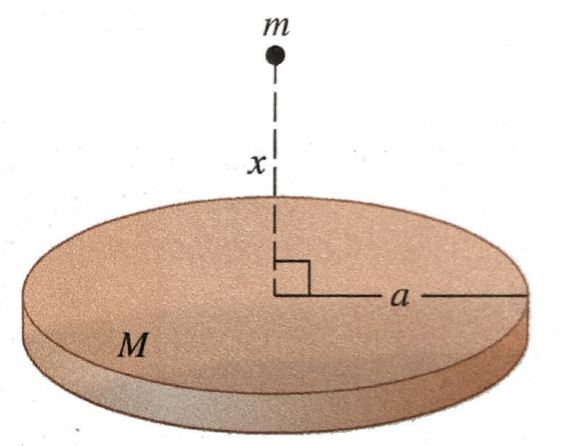
\includegraphics[width=5.5cm]{../figures/A2_2.png}
  \caption{}
  \label{fig:A2_2}
\end{wrapfigure}

Mass $M$ is distributed uniformly over a disk of radius $a$. Find the gravitational force (magnitude and direction) between this disk-shaped mass and a particle with mass $m$ located a distance $x$ above the center of the disk \textbf{\autoref{fig:A2_2}}. Does your result reduce to the correct expression as $x$ becomes very large? (\textit{Hint:} Divide the disk into infinitesimally thin concentric rings, use the expression derived in Exercise 13.39 for the gravitational force due to each ring, and integrate to find the total force.)

\bigbreak

\begin{figure}[ht]
  \centering
  \incfig[0.4]{A2_3}
  \caption{Tegning af \textit{disken} samt en enkelt af de tynde ringe som \textit{disken} opdeles i.}
  \label{fig:A2_3}
\end{figure}

Først opdeles \textit{disken} i en række tynde ringe, med radius $r$ og tykkelse $\mathrm{d}r$ som vist på \textbf{\autoref{fig:A2_3}}. Fra \textit{Exercise 13.39} har vi at kraftpåvirkningen på partiklen med masse $m$ fra en ring med masse $\mathrm{d}m$ og radius $r$ er givet ved
\begin{equation} \label{eq:1}
    \mathrm{d}F = - \frac{G \cdot m \cdot \mathrm{d}m \cdot x}{\left( x^2 + r^2 \right)^{\frac{3}{2}}}
\end{equation}
Vi ønsker nu at finde et udtryk for massen af de infinitesimalt tynde ringe, $\mathrm{d}m$. Arealet af en af ringene kan findes som forskellen mellem arealet af den cirkel der udgør den yderste kant med radius $r + \mathrm{d}r$ og arealet af den cirkel der udgør den inderste kant med radius $r$. Altså har vi at
\begin{align*}
  A_{ring} &= \pi(r + \mathrm{d}r)^2 - \pi(r)^2 \\
           &= \pi \cdot r^2 + 2 \pi \cdot r \, \mathrm{d}r + \pi(\mathrm{d}r)^2 - \pi \cdot r^2 \\
           &= 2\pi \cdot r \, \mathrm{d}r + \pi(\mathrm{d}r)^2
.\end{align*}
For $\mathrm{d}r \to 0$ bliver $(\mathrm{d}r)^2 \ll 2r \cdot \mathrm{d}r$ og vi kan derfor approksimere arealet af en ring som
\[ 
A_{ring} = 2\pi \cdot r \, \mathrm{d}r
.\]
Densiteten pr. areal-enhed af hele \textit{disken} må være dens masse over dens areal så
\[ 
\rho_A = \frac{M}{\pi a^2}
.\]
Og massen af en af de infinitesimalt tynde ringe må derfor være
\[ 
  \mathrm{d}m = A_{ring} \cdot \rho_A = \rho_A(2\pi r \, \mathrm{d}r)
.\]
Dette kan nu substitueres ind i (\ref{eq:1}) så vi får at
\[ 
  \mathrm{d}F = - \frac{Gm\rho_A(2\pi r \, \mathrm{d}r)x}{\left( x^2 + r^2 \right)^{\frac{3}{2}}}
.\]
For at finde den samlede kraftpåvirkning fra alle ringene integreres over hele \textit{disken}, dvs. fra $r = 0$ til $r = a$. Dermed kan følgende integral opskrives
\begin{align*}
  \int_{0}^{a} \mathrm{d}F &= \int_{0}^{a} - \frac{Gm\rho_A(2\pi r \, \mathrm{d}r)x}{\left( x^2 + r^2 \right)^{\frac{3}{2}}} \\
  F &= \int_{0}^{a} - \frac{Gm\rho_A(2\pi r \, \mathrm{d}r)x}{\left( x^2 + r^2 \right)^{\frac{3}{2}}} \\
  &= -2\pi G m \rho_A x \int_{0}^{a} \frac{r \, \mathrm{d}r}{\left( x^2 + r^2 \right)^{\frac{3}{2}}}
.\end{align*}
Vi ønsker derfor at løse integralet
\[ 
\int_{0}^{a} \frac{r \, \mathrm{d}r}{\left( x^2 + r^2 \right)^{\frac{3}{2}}}
.\]
Integralet løses vha. substitution. Vi sætter $u = x^2 + r^2$, hvilket giver $\mathrm{d}u = 2r \, \mathrm{d}r$. For $r = 0$ bliver integrationsgrænsen $x^2$ og for $r = a$ bliver integrationsgrænsen $x^2 + a^2$. Altså bliver integralet
\begin{align*}
  \int_{x^2}^{x^2 + a^2} \frac{1}{2u^{\frac{3}{2}}} \, \mathrm{d}u &= \left[ - \frac{1}{\sqrt{u}} \right]_{x^2}^{x^2 + a^2} \\
  &= -\frac{1}{\sqrt{x^2 + a^2}} - \left( - \frac{1}{\sqrt{x^2}} \right) \\
  &= -\frac{1}{\sqrt{x^2 + a^2}} + \frac{1}{x}
.\end{align*}
Dette kan nu substitueres tilbage ind i vores udtryk fra før så
\[ 
F = -2\pi G m \rho_A x \left(- \frac{1}{\sqrt{x^2 + a^2}} + \frac{1}{x} \right)
.\]
Og udtrykket for densiteten pr. areal-enhed $\rho_A$ kan også substitueres ind så vi får at
\begin{align*}
  F &= \frac{-2\pi G m M x}{\pi a^2} \left( - \frac{1}{\sqrt{x^2 + a^2}} + \frac{1}{x} \right) \\
    &= \frac{-2 G m M}{a^2} \left( \frac{x}{x} - \frac{x}{\sqrt{x^2 + a^2}} \right) \\
    &= \frac{-2 G m M}{a^2} \left( 1 - \frac{x}{\sqrt{x^2 + a^2}} \right)
.\end{align*}
Altså bliver den samlede gravitationskraft på massen $m$ fra \textit{disken} \underline{\underline{$F = -\frac{2G m M}{a^2} \left( 1 - \frac{x}{\sqrt{x^2 + a^2}} \right)$}}. Det bør bemærkes at fortegnet angiver at kraften er i retningen fra massen $m$ mod \textit{disken}. For at undersøge, hvordan udtrykket reagerer for store afstande, $x \gg a$ betragter vi brøken
\[ 
\frac{x}{\sqrt{x^2 + a^2}} = \frac{x}{x \sqrt{1 + \frac{a^2}{x^2}}} = \frac{1}{\sqrt{1 + \frac{a^2}{x^2}}}
.\]
For $x \gg a$ bliver værdien af $\frac{1}{\sqrt{1 + \frac{a^2}{x^2}}}$ meget tæt på, men lidt mindre end 1. Vi indfører $\epsilon = \frac{a^2}{x^2}$ og får dermed følgende udtryk
\[ 
  \frac{1}{\sqrt{1 + \epsilon}}
.\]
Dette approksimeres vha. 1.-grads Taylor-polyonimet for $\frac{1}{\sqrt{1 + \epsilon}}$ ved $\epsilon = 0$.
\begin{align*}
  \frac{1}{\sqrt{1 + \epsilon}} &\approx f(0) + f'(0)\epsilon \\
  &= 1 - \frac{1}{2} \epsilon \\
  &= 1 - \frac{a^2}{2x^2}
.\end{align*}
Bemærk, at denne approksimation kun er gyldig for små værdier af $\epsilon$, hvilket også er tilfældet for $x \gg a$. Dette kan nu sættes tilbage ind i udtrykket for den samlede kraft, så vi får at
\begin{align*}
  F &\approx - \frac{2 G m M}{a^2} \left( 1 - \left( 1 - \frac{a^2}{2x^2} \right) \right) \\
    &= - \frac{2G m M}{a^2} \left( \frac{a^2}{2x^2} \right) \\
    &= - \frac{G m M}{x^2}
.\end{align*}
Dette er den velkendte formel for gravitationskraften mellem to punktmasser og dermed er det vist, at \underline{\underline{udtrykket giver den rigtige værdi}} for en stor afstand $x$.


\section*{Problem 3/3}
Example 13.10 assumes a constant density for the earth, but Fig. 13.9 shows that this is not accurate.

\subsection*{(a)}
Approximate the density graph in Fig 13.9 by a straight line running from \qty{13000}{kg/m^3} at $r = 0$ to \qty{3000}{kg/m^3} at $r = R_E$. Divide the earth into concentric shells of width $\mathrm{d}r$ and therefore volume $\mathrm{d}V = 4\pi r^2 \, \mathrm{d}r$. Integrate to find the mass enclosed as a function of the distance from the earth's center.
\bigbreak
Først opskrives et udtryk for densiteten af jorden, $\rho$, som funktion af afstanden til jordens midte, $r$. Hertil benyttes blot formlen for en ret linje igennem to punkter, idet to punkter er angivet. Altså fås densitetsfunktionen $\rho(r)$ som
\[ 
  \rho(r) = \rho(0) + \left( \rho(R_E) - \rho(0) \right) \frac{r}{R_E} = \qty{13000}{\frac{kg}{m^3}}  - \qty{10000}{\frac{kg}{m^3}}  \frac{r}{R_E}
.\]
Jorden inddeles i tynde kugleskaller, som beskrevet i opgaven og disse kugleskaller får derfor hver i sær et volumen på 
\[ 
  \mathrm{d}V = 4\pi r^2 \, \mathrm{d}r
.\]
For at finde massen af en kugleskal benyttes det faktum at masse er produktet af densitet og volumen så vi får at
\[ 
  \mathrm{d}m = \rho(r) \, \mathrm{d}V = 4\pi \left( \qty{13000}{\frac{kg}{m^3}} r^2 - \qty{10000}{\frac{kg}{m^3}}   \frac{r^3}{R_E}  \right) \, \mathrm{d}r
.\]
Vi ønsker at finde den totale masse $M(d)$ som er \textit{enclosed} i en kugleskal med radius $d$. Altså integreres fra $r = 0$ til $r = d$ så
\begin{align*}
  \int_{0}^{d} \, \mathrm{d}m &= 4\pi \int_{0}^{d} \left( \qty{13000}{\frac{kg}{m^3}}   r^2 - \qty{10000}{\frac{kg}{m^3}}  \frac{r^3}{R_E} \right) \, \mathrm{d}r \\
  M(d) &= 4\pi \left[ \qty{13000}{\frac{kg}{m^3}}  \frac{r^3}{3} - \qty{10000}{\frac{kg}{m^3}}  \frac{r^{4}}{4R_E} \right]_{0}^{d} \\
  &= 4\pi \left( \qty{13000}{\frac{kg}{m^3}}  \frac{d^3}{3} - \qty{10000}{\frac{kg}{m^3}}  \frac{d^{4}}{4R_E} \right) \\
  &= \frac{4\pi d^3}{3} \left( \qty{13000}{\frac{kg}{m^3}}  - \frac{\qty{7500}{\frac{kg}{m^3}} d}{R_E}  \right)
.\end{align*}
Altså er massen $M$ \textit{enclosed} i en kugleskal med radius $d$, \underline{\underline{$M(d) = \frac{4\pi d^3}{3} \left( \qty{13000}{\frac{kg}{m^3}}  - \frac{\qty{7500}{\frac{kg}{m^3}} d}{R_E} \right)$}}.


\subsection*{(b)}
Find the expression for the magnitude of the gravitational force on a mass $m$ at a distance $r$ from the earth's center.
\bigbreak
I denne opgave ønsker vi at benytte $r$ som vores afstand til jordens massemidtpunkt, dette svarer til integrationsgrænsen, $d$ fra sidste opgave og derfor vil det følgende bruge $r$ i stedet for $d$ og $M(r)$ i stedet for $M(d)$. Grunden til at $d$ blev introduceret i sidste opgave var blot for at undgå at bruge integrationsvariablen som integrationsgrænse.  Vi opskriver først Newtons tyngdelov
\[ 
  F = \frac{GMm}{r^2}
.\]
Vi indsætter udtrykket for massen af jorden fra sidste opgave på $M$'s plads så
\begin{align*}
  F &= \frac{Gm}{r^2}M(r) \\
  &= \frac{Gm}{r^2} \cdot \frac{4\pi d^3}{3} \left( \qty{13000}{\frac{kg}{m^3}} - \frac{\qty{7500}{\frac{kg}{m^3}}r}{R_E} \right) \\
  &=  \frac{4\pi G m r}{3} \left( \qty{13000}{\frac{kg}{m^3}} - \frac{\qty{7500}{\frac{kg}{m^3}} r}{R_E} \right)
.\end{align*}
Altså bliver gravitationskraften på en masse $m$ placeret en afstand $r$ fra jordens centrum \underline{\underline{$F = \frac{4\pi G m r}{3} \left( \qty{13000}{\frac{kg}{m^3}} - \frac{\qty{7500}{\frac{kg}{m^3}} r}{R_E} \right)$}}.

\end{document}
